
\documentclass[tightpage, 26pt]{standalone}
\usepackage{tikz}

\usetikzlibrary{decorations.text}

\newcommand{\drawsector}[6][]{
    \draw[#1] (#4:{#2-.5*#3}) arc [start angle = #4, delta angle=-#5, radius={#2-.5*#3}]--++({#4-#5}:#3) arc [start angle = {#4- #5}, delta angle=#5, radius={#2+.5*#3}] --cycle;
\draw[decorate,decoration={raise=-3pt, text along path, text=#6, text align={align=center}}] (#4:#2) arc(#4:(#4-#5):#2);
}


\begin{document}
 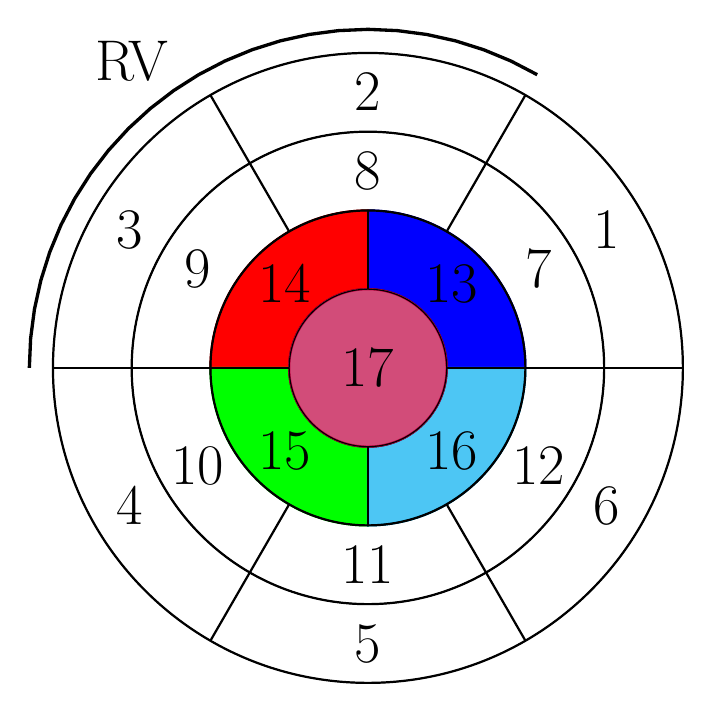
\begin{tikzpicture}\tikzstyle{every node}=[font=\huge]

   \drawsector[draw=blue, thick, fill=blue]{1.5cm}{1cm}{90}{90}{}
   \drawsector[draw=red, thick, fill=red]{1.5cm}{1cm}{180}{90}{}
   \drawsector[draw=green, thick, fill=green]{1.5cm}{1cm}{270}{90}{}
   \drawsector[draw=cyan, thick, fill=cyan!70]{1.5cm}{1cm}{360}{90}{}
     
   % Circles 
    \foreach \r in {1, 2,3,4}
      \draw[black, thick] (0,0) circle (\r) ;

   % Fill cirlces
    \draw[draw=purple, thick, fill=purple!70] (0,0) circle (1cm);
    \draw[] (0,0) circle (2cm) (0:1) arc (0:-360:1) ;
    \draw[] (0,0) circle (3cm) (1:2) arc (1:-360:2) ;
    \draw[] (0,0) circle (4cm) (2:3) arc (2:-360:3) ;
    
    % Rays
    \foreach \a in {0, 180}
      \draw[thick,black] (\a:1) -- (\a:4);   

    \foreach \a in {90, 270}
      \draw[thick,black] (\a:1) -- (\a:2);

    \foreach \a in {60, 120, 240, 300}
      \draw[thick,black] (\a:2) -- (\a:4); 



    % Draw numbers
    \draw[black, thick] (0,0) node{$17$};

    \foreach \a in {13,14,15,16}
      \draw[black, thick] (-1125+ 90*\a:1.5) node{$\a$};
      % 45 + 90*(\a-13) = -1125 + 90*\a

    \foreach \a in {7,8,9,10,11,12}
      \draw[black, thick] (-390+ 60*\a:2.5) node{$\a$};
      % 30 + 60*(\a-7) = -390 + 60*\a

    \foreach \a in {1,2,3,4,5,6}
      \draw[black, thick] (-30+ 60*\a:3.5) node{$\a$};
      % 30 + 60*(\a-1) = -30 + 60*\a

    % Draw RV
    \draw [black,very thick,domain=60:180] plot ({4.3*cos(\x)}, {4.3*sin(\x)});
    \draw[black, thick] (-3.0,3.9) node{RV};

\end{tikzpicture}


\end{document}
%%% Local Variables:
%%% mode: latex
%%% TeX-master: t
%%% End:
